%\documentclass[aps,onecolumn,preprintnumbers,amsmath,amssymb,nofootinbib,superscriptaddress,notitlepage]{revtex4-1}
%\documentclass[preprint,12pt]{elsarticle}
\documentclass[5p,times]{elsarticle}
%\documentclass[aps,nofootinbib,prl,showpacs,twocolumn,groupedaddress,superscriptaddress]{revtex4}


\usepackage{graphicx}
\usepackage{dashrule}
\usepackage{dcolumn}
\usepackage{mathtools}
\usepackage{amssymb}
\usepackage{bbold}
\usepackage{amsmath}
\usepackage{amsfonts}
\usepackage{wasysym}
\usepackage{slashed}
\usepackage[dvipsnames]{xcolor}
\usepackage{soul}
\usepackage{rotating}
\usepackage{paracol}
\usepackage{nicefrac}
\usepackage{MnSymbol}

%\usepackage{subcaption}
%\newbox{\bigpicturebox}

\newcommand{\reales}{{\rm R}\hspace{-1ex}\rule{0.1mm}{1.5ex}\hspace{1ex}}
\def\tstrut{\vrule height2.5ex depth0pt width0pt} % used in tables
\def\jtstrut{\vrule height5ex depth0pt width0pt} % used in tables

\newcommand{\figref}[1]{fig.~(\ref{#1})}
\newcommand{\tabref}[1]{table~(\ref{#1})}
\newcommand{\ccite}[1]{ref.~\cite{#1}}

\newcommand{\eref}[1]{eq.~(\ref{#1})}
\newcommand{\eg}{\textit{e.g.}~}
\newcommand{\ie}{\textit{i.e.}~}
\newcommand{\viz}{\textit{viz.}~}
\newcommand{\cf}{\textit{cf.}~}
\newcommand{\eftnopi}{\mbox{EFT($\slashed{\pi}$) }}
\newcommand{\ve}[1]{\ensuremath{\boldsymbol{#1}}}
\newcommand{\rcm}{\ensuremath{\ve{R}_\text{\scriptsize{c.m.}}}}
\newcommand*{\mprime}{^{\prime}\mkern-1.2mu}
\newcommand*{\mdprime}{^{\prime\prime}\mkern-1.2mu}
\newcommand*{\mtprime}{^{\prime\prime\prime}\mkern-1.2mu}
\newcommand{\ddrei}[1]{\delta_{\tiny \lambda}^{(3)}\!\big(#1\big)}
\newcommand{\cc}{\ensuremath C(\lambda)}
\newcommand{\dd}{\ensuremath D(\lambda)}
\newcommand{\hbstwom}{\ensuremath \frac{\hbar^2}{2\mu}}
\newcommand{\twomhbs}{\ensuremath \frac{2\mu}{\hbar^2}}
\newcommand{\coup}[3]{\left[\,#1\,\otimes\,#2\,\right]^{#3}}
\newcommand{\threej}[6]{ \begin{pmatrix}
   #1 & #2 & #3 \\
   #4 & #5 & #6
  \end{pmatrix}}

\newcommand{\bra}[1] {\left\langle~#1~\right|}
\newcommand{\ket}[1] {\left|~#1~\right\rangle}
\newcommand{\bet}[1] {\left|#1\right|}
\newcommand{\overlap}[2] {\left\langle\,#1\,\left|\,#2\,\right.\right\rangle}
\newcommand{\me}[3] {\left\langle\,#1\,\left.\left|\,#2\,\right|\right.\,#3\,\right\rangle}
\newcommand{\mer}[3] {\left\langle\,#1\,\left|\left.\,#2\,\right|\,#3\,\right.\right\rangle_{\ve{R}}}
\newcommand{\redme}[3] {\left\langle\,#1\,\middle|\right|\,#2\,\left|\middle|\,#3\,\right\rangle}

\definecolor{green}{HTML}{2E8B57}
\interfootnotelinepenalty=10000 %% Completely prevent breaking of footnote

\usepackage{xcolor}
\colorlet{darkgreen}{green!50!black}
\colorlet{brightyellow}{yellow!75!red}
\colorlet{orange}{red!50!yellow} \colorlet{darkred}{red!80!black}
\colorlet{darkblue}{blue!50!black}

\usepackage{soul}
\newcommand{\remove}[1] {\textcolor{darkred}{\st{#1}}}
\newcommand{\comment}[2] {\textcolor{green}{[\textbf{comment - #1}: {#2}]}}
\newcommand{\remark}[2] {\textcolor{orange}{[\textbf{\textsf{remark - #1}}: {\textsf{#2}}]}}
\newcommand{\highlight}[1] {\textcolor{red}{{#1}}}
\newcommand{\repl}[2] {\textcolor{darkred}{\st{#1}}\textcolor{blue}{#2}}
\newcommand{\place}[1] {\textcolor{blue}{{#1}}}
\newcommand{\edit}[1] {\textcolor{red}{{#1}}}

\begin{document}



\title{Emergence of $^4$H $J^\pi=1^-$ resonance in contact theories}

\author{Lorenzo Contessi}%\email{lorenzo@contessi.net}
\address{Universit\'e Paris-Saclay, CNRS-IN2P3, IJCLab, 91405 Orsay, France}
\address{IRFU, CEA, Universit\'e Paris-Saclay, 91191 Gif-sur-Yvette, France}

\author{Martin Sch{\"a}fer}
\address{The Racah Institute of Physics, The Hebrew University, Jerusalem 9190401, Israel}

\author{Johannes Kirscher}
\address{Department of Physics, SRM University - AP, Amaravati 522502, Andhra Pradesh, India}

\author{Rimantas Lazauskas}
\address{IPHC, IN2P3-CNRS/Universit\'e de Strasbourg BP 28, F-67037 Strasbourg Cedex 2, France}

\author{Jaume Carbonel}
\address{Universit\'e Paris-Saclay, CNRS/IN2P3, IJCLab, 91405 Orsay, France}




\date{\today}



\begin{abstract}

Elastic neutron-triton scattering is considered at leading order in pionless effective field theory.
In the infinite-cutoff limit, we obtain the scattering length $a_0(\infty) = 3.06(1)$~fm
and the effective range $r_0(\infty) = 1.59(7)$~fm ($S$-wave). 
In the $P$-wave channel, we predict a scattering volume $a_1(\infty) = -9.8(1.6)$~fm$^3$
and a range equivalent $r_1(\infty) = 1.3(4)$~fm$^{-1}$ with the same zero-range theory. 
%
The results are extracted with three numerical techniques: a
Gaussian-stochastic-variational method, an integration of the configuration-space Faddeev-Yakubovsky 
equations, and a resonating-group reduction of the four-body problem to an effective two-body cluster theory. 
Renormalization-group dependence is assessed through variation of a cutoff regulator parametrized in a
range between $1\,\text{fm}^{-1}$ and $10\,\text{fm}^{-1}$.
%
Most remarkably, we find a cutoff-stable/RG-invariant resonance in the $^4$H $J^\pi=1^-$ system.
This $P$-wave resonance is thus a universal consequence of the unitary deuteron system
and an ensuing discretely scale invariant three-body system with a scale set by the triton binding energy.
%
This stabilization of a resonant state in a few-fermion system solely through pure contact interactions
has a significant consequences for the powercounting of the pionless theory.
Specifically, the existence of a resonance implies that the known inability of the theory's leading order
to bind larger nuclei like 16-oxygen can be cured in perturbation theory.
\end{abstract}

\maketitle

%================================================
\section{Introduction}
%================================================

Contact effective field theory (EFT) is not only practical in describing
bosonic~\cite{Bazak:2016wxm,Carlson:2017txq,Bazak:2018qnu,Bedaque:1998kg,Bedaque:1998km} 
and few-nucleon~\cite{Bedaque:1999ve,Barnea:2013uqa} systems, it represents a systematic
expansion of the underlying scales and their interactions~\cite{Hammer:2019poc,Barnea:2013uqa}, and
thereby provides a transparent framework to study the emergence of many-body phenomena from few-body properties.
However, the nuclear incarnation of such a theory, Pionless effective field theory (\eftnopi), apparently fails to predict
stable bound states for $P$-shell
nuclei\footnote{Fermi systems with more particles than accessible internal states}
at the leading order (LO)~\cite{Stetcu:2006ey,Contessi:2017rww,Dawkins:2019vcr,Schafer:2020ivj}. 
%
For instance, the lightest of such nuclei, $^6 {\rm Li}$, is 
found unstable with respect to breakup into $\rm ^4He$ in its ground state ($\alpha$)
and a deuteron ($d$) in the zero-range contact limit~\cite{Schafer:2020ivj}~of LO~\eftnopi.
Whether or not the theory finds the physical bound state at LO veiled as a virtual or resonant state which
reveals its physical character at higher orders is arguably the most imminent problem of the development of contact EFTs for
Fermi systems.
As perturbative higher-order insertions cannot create poles {\it ex novo}, the conceivable absence of such poles
within the convergence radius of LO~\eftnopi~would make the theory in its current version useless for the description
of larger nuclei.
The challenge cast in simple words: Does the LO~\eftnopi~support any type of non-zero poles at complex momenta below its
breakdown scale?

Historically, resonances were studied in (A$\le$4)-body bosonic systems close to the unitary limit\cite{Deltuva:2012ig,deltuva2020energies} confirming the existence of a tower of Efimov resonances. 
A recent study\cite{Habashi:2020qgw} proved the possibility of creating two-body $S$-shell resonances in the contact limit with negative effective range.%, naidon2017efimov}. 
In the \eftnopi at LO framework, a resonance have been also found in neutral hypernuclear system $\Lambda nn$ \cite{Schafer:2020rba} and $S$-wave virtual states have been confirmed as exited states of triton \cite{Rupak:2019} and hypertriton \cite{Schafer:2020rba}. 
Finally, a recent study of $^3n$ confirmed the absence of $P$-wave resonance or virtual state in this system\cite{Dietz:2021haj}. 
At the present knowledge of the authors, the calculations of $P$-shell systems stops at this level and no studies have been done for discrete invariant systems of equal mass.
The major goal of this work is to study resonances in $^4$H a system never addressed before in this framework and that can be understood starting from its universal behavior. 
The existence of an eventual $P$-shell resonance using \eftnopi at LO would open the possibility of finding the same structure also in heavier nuclei, with the chance of stabilizing many-nucleon systems by perturbative corrections.
%

%
Experimentally, $^4$H resonances are clearly seen in n-$^3$H elastic cross sections \cite{PhysRev.119.1981,SEAGRAVE1972250}, as well as in $\pi^-$ absorption experiments \cite{Sennhauser:1981tr,Gornov:1991fg}, or in transfer reactions \cite{Miljanic:1986zz,Sidorchuk:2003fwa}. 
However, extracted resonance parameters differ substantially, depending on the used protocol and on the underlying hypothesis in the data analysis. 
For instance, results of the same $\pi^-$+$^9$Be$\,\to\,$d+t+$^4$H experiment, performed by the same authors, yields for the lowest state ($E_R$=3.0$\pm$0.2~MeV, $\Gamma$=4.7$\pm$1~MeV) \cite{Gornov:1991fg}, ($E_R$=2.0$\pm$0.2~MeV, $\Gamma$=1.2$\pm$0.2~MeV) \cite{Gurov:2005sp}, and ($E_R$=1.6 $\pm$0.1 MeV, $\gamma^2$=0.4$\pm$0.1~MeV)\cite{Gurov2005p}, where $\gamma$ is the reduced width (see the original paper), depending whether one assumes the experimental signal to be created respectively by one, two, or three resonant states.
Independently, the $R$-matrix analysis of n-$^3$H cross section \cite{Tilley:1992zz} concluded about a superposition of several $P$-waves resonant states with quantum numbers $J^\pi$=$0^-$,$1^-$,$2^-$. 
With two non-degenerate $J^\pi$=$1^-$ states (denoted $1^-_I$ and $1^-_{II}$ ) corresponding to two different total spin contributions in the asymptotic channels\cite{Lazauskas:2004uq}. 
The lowest state parameters found in this case ($E_R$=3.2 MeV, $\Gamma$=5.4 MeV) are hardly compatible with the previous many-state analysis. 
The discrepancies among different experimental approaches further
increase when including the transfer reaction experiments.
%

From a numerical point of view, computing the $S$-matrix pole of a resonance is not an easy task. 
Microscopic ab initio calculations for nuclear few-body systems are therefore not abundant and up to now have been performed for a limited amount of particles ($A<6$) \cite{Li:2019pmg,Lazauskas:2019cxj}. 
This limit is often circumvented by changing the calculation
degrees of freedom and treating the many-body systems as a few-body problem between clusters as done in Ref.~\cite{Arai:2003ek,deDiego:2007rd} introducing approximations in the solution \cite{doweneedthis}.
Resonances in $^4$H have been studied in the past, for example, in Ref.~\cite{deDiego:2007rd} using an effective two-body n-$^3$H potential adjusted to reproduce the $p$-$^3$He experimental phase shifts. 
Here, the resonance energy has been calculated either directly computing the $S$-matrix pole or by performing a $R$-matrix analysis of the phase shifts, showing a sensible difference among the two methods (the $1^-_I$ resonance is located at energy $E_r=1.2$, $\Gamma=3.5$ MeV, and $E_r=3.6$, $\Gamma=5.3$ MeV respectively).
%
% I dont know why this was removed, but it is the main point of the above paragraph
This result further enhances the difference between the position of the S-matrix pole and the resonance position extracted from the cross section, making difficult any kind of comparison between different calculations and experiments.
%
Other calculations have been done in Refs.~\cite{Arai:2003ek,Horiuchi:2013iw,Lazauskas:2019cxj,Li:2021ado} using the resonating group method (RGM) with complex scaling, Spin-dipole strength functions, Faddeev-Yakubowski equations (FYE) in configuration space, and No-core Gamov Shell Model. The results differs from method to method varying in a range $E_R=\{0.9-3.6\}$ MeV and $\Gamma=\{1.0-5.3\}$ MeV.
This variation appears to be a consequence of the different numerical techniques used more than on the interaction employed. In fact, studying the position of the resonance with different realistic interactions but the same theoretical scheme \cite{Lazauskas:2019cxj,Li:2021ado} leads to comparable results.

%
%

In this letter, we study the emergence of a 3+1 $J^{\pi}=1^-$ resonance in $^4$H using LO \eftnopi, demonstrating the possibility of creating n$^3$H $P$-wave states using a purely $S$-wave contact interaction. 
In the region of resonance projectile neutron momentum is $\sim 0.5~m_\pi$, binding momenta of nucleons within $^3$H target are $\sim 0.4~m_\pi$ (for a combined distance from the complete disintegration threshold of $0.8~m_\pi$): thus $^4$H resonant states are at the limit of convergence of \eftnopi, nevertheless still observable in a LO calculation. The absence of any spin-orbit or tensor term in the LO interaction causes degeneracy between $J^{\pi}=0,^-,1^-_I,1^-_{II},2^-$ states which would be splitted including higher orders. 
As $^4$H can still be treated as both a four-body and two-cluster (triton-neutron) system, we choose to employ both the methodologies starting from the same nuclear Hamiltonian.

%================================================
\section{Theory and numerical methods}
%================================================

The theory used in this work is the \eftnopi\cite{vanKolck:1999mw} truncated at LO. The lowest order consists of contact two-body and a contact three-body interactions with corresponding low energy constants (LECs) fitted to reproduce physical observables. To further simplify the theory we truncate it around the SU(4) symmetry \cite{Konig:2016utl}. %the theory is perturbative around su(4) symmetry, so we do not assume but we truncate it
Therefore, $NN$ spin-singlet and spin-triplet interactions are identical and only one contact term appears in the two-body sector. This adds further uncertainty to the theory of order $(a_0m_{\pi})^{-1}\sim30\%$ on the top of the usual \eftnopi LO truncation error. The contact interactions are regularized by an introduction of a Gaussian regulator and a momentum cut-off $\Lambda$. This yields two- and three-body potential 
%
\begin{equation}
    V(\textbf{r})=C_0 \sum_{i,j}^N e^{-\frac{r_{ij}^2\Lambda^2}{4}},
\end{equation}
%
\begin{equation}
    W(\textbf{r})=D_0 \sum_{ijk}^N \left[
    e^{-\frac{(r_{ij}^2+r_{ik}^2)\Lambda^2}{4}}+
    e^{-\frac{(r_{ij}^2+r_{jk}^2)\Lambda^2}{4}}+
    e^{-\frac{(r_{jk}^2+r_{ik}^2)\Lambda^2}{4}}\right],
\end{equation}
%
where the cut-off dependent LECs ($C_0$ and $D_0$) are fitted on two-body observables and triton binding energy ($B_3=8.48$~MeV). 
In order to assess the uncertainty introduced by the adoption of SU(4) symmetry, we use two different parametrizations for the two-body LEC $C_0$: one at unitarity (with $|a_0|>10^5$~fm and referred to as ``unitary'') and one fitting the deuteron binding energy $B_2=2.22$~MeV (referred as ``nuclear''). We assume a degenerate nucleon mass $m=938.858$ MeV.

To extract the effective range parameters and resonance energy we employ and compare results of three different methods. We use two ab initio techniques (four-body calculations): the direct solution of the Faddeev-Yakubovsky equations (FYE) in configuration space \cite{Lazauskas:2004hq, Lazauskas:2019hil} and the stochastic variational methods (SVM)\cite{Suzuki:1998bn}; 
and a potential folding technique that reduces the problem into effective two-body problem, represented by neutron impinging on a solid triton core.

Employing the above interaction we extract the triton-neutron scattering parameters ($a_L$ and $r_L$) for $L=0$ and $L=1$ trough the effective range expansion (ERE) expanded around the triton-neutron threshold:
%
\begin{equation}
    k^{2L+1}\text{cot}(\delta_L)=-\frac{1}{a_L}+\frac{1}{2}r_L k^2 + ... \, ,
    \label{eq.app.ere}
\end{equation}
%
where $\delta_L$ is the triton-neutron phase-shift at angular momentum $L$ and $k$ is the center of mass momentum of the fragments. 
Resonances will, therefore, emerge as poles of the system's $T$-matrix
%
\begin{equation}
T =\frac{4\pi}{m}\frac{1}{\text{cot}(\delta)-i} =
\frac{4\pi}{m}\frac{k^{2L+1}}{\frac{1}{a_L}+...+\frac{1}{2}r_L k^2
-ik^{2L+1}} \label{eq:Tmatrix}
\end{equation}
%
and can be extracted either by fitting phase shifts to the ERE formula or directly through solving the Schr\"odinger equation for complex energies.
%
From an theoretical point of view, extracting the resonance energy with the two methods is not equivalent. 
Solving the Schr\"odinger equation for complex energies is affected by the \eftnopi LO truncation error ($\Gamma_{\eftnopi}\approx k_{res}/m_\pi\sim80\%$), while extracting the resonance position using the ERE of the triton-neutron phaseshift and using RGM formalism (see below) is equivalent to the halo-EFT expanded around t-n treshold.
In the latter case, a new scale, the breaking momentum of $^3$H, is introduced at momentum $K_{d-n}\simeq94$ MeV. 
Since the scattering parameters are extracted using \eftnopi at LO we expect the two methods to agree inside the truncation error $\Gamma_{Halo}\approx k^*_{res}/K_{d-n}\simeq70\%$ using only the scattiring volume and $\Gamma_{Halo}^2$ %should be square, but if someone recheck is better
if the effective range $r_1$ is also included in the ERE.

\vspace{2mm}



%================================================
\subsection{Faddeev-Yakubovsky equation formalism}
%================================================

This formalism, as well as our employed numerical techniques, have been described in detail in Refs.~\cite{Lazauskas:2004hq,Lazauskas:2019hil}.
Here we will just stress that, in order to determine n-$^3$H scattering lengths (volumes), we solve the differential FYE equations by requiring the systems wave function to satisfy boundary condition in the far asymptote for retrieving neutron, defined by:
%
\begin{equation}
\begin{split}
\Psi(X_{^3{\rm H}},\vec{y}_{n-^3{\rm H}})=&\lim_{k\rightarrow0}\psi_t(X_{^3{\rm H}})\big([j_L(k|y_{n-^3{\rm H}}|)/k^{L}]\\
&+a_L(k) [n_L(k|y_{n-^3{\rm H}}|)k^{L+1}]\big)Y_L(\hat{y}_{n-^3{\rm H}});  \label{eq:FYe_a}
\end{split}
\end{equation}
%
here $j_L(z)$ and $n_L(z)$ are spherical Bessel functions of the first and second kind respectively. 
$\psi_t(X_{^3{\rm H}})$ is the wave function of the $^3$H ground state, which is found before undertaking n-$^3$H scattering calculations. 
In the particular case of determining the scattering lengths (volumes) $a_L$, calculations are performed for vanishing momenta $k$.
Note that, in the limit $k\rightarrow0$, the expressions in the brackets are finite functions depending on a distance $|y_{n-^3{\rm H}}|$.

To determine positions of the resonant states we solve FYE by imposing slightly different boundary condition for neutron asymptote:
\begin{equation}
\begin{split}
\Psi(X_{^3{\rm H}},\vec{y}_{n-^3{\rm H}})=&\psi_t(X_{^3{\rm H}}) \big(h_L^+(k_{r}|y_{n-^3{\rm H}}|)\\
&+F_L(k_r)h_L^-(k_{r}|y_{n-^3{\rm H}}|)\big) Y_L(\hat{y}_{n-^3{\rm H}});  \label{eq:FYe_res}
\end{split}
\end{equation}
here $h_L^-(z)$ and $h_L^+(z)$ are Spherical Bessel functions of the third kind. Complex momentum plane $k_r$ is scanned to find positions where the function $F_L(k_r)$ vanishes and thus wave function $\Psi(X_{^3{\rm H}},Y_{n-^3{\rm H}})$ represents purely outgoing n-$^3$H waves.
 
%================================================
\subsection{Harmonic oscillator trap}
%================================================
The second microscopic approach involves an introduction of the Harmonic oscillator (HO) trapping potential
\begin{equation}
    V_{\rm HO}(\textbf{r}) = \frac{m}{2A} \omega^2 \sum_{i<j} (\textbf{r}_i - \textbf{r}_j)^2
\end{equation}
with oscillator frequency $\omega$ into $A=4$-body $^4$H system.

Assuming that the range of an interaction is much smaller than the typical HO trap range $R << b_{\rm HO} =\sqrt{2/(m \omega)}$ one can match asymptotic $n ^3$H part of a trapped $^4$H wavefunction to the trapped solution of effective $n ^3$H two-body system with no nuclear interaction considered. The $n ^3$H phasehifts $\delta_L$ at relative momentum $k$ are then extracted using generalized Bush formula for an arbitrary orbital momentum $L$ \cite{Suzuki:2009}    

\begin{equation}
    (-)^{L+1} \left(\sqrt{4\mu \omega}\right)^{2L+1} \frac{\Gamma\left(3/4 + L/2 - \epsilon^n_\omega/2\omega\right)}{\Gamma\left(1/4 - L/2 - \epsilon^n_\omega/2\omega\right)} = k^{2L+1}~{\rm cot}\left(\delta_L \right),
\end{equation}
where $ k=\sqrt{2\mu \epsilon^n_\omega}$, $\Gamma(x)$ is a Gamma function, $\mu \simeq 3/4 m$ denotes $n ^3$H reduce mass, and $\epsilon^n_\omega = E_\omega (^4{\rm H})-E_\omega (^3{\rm H})$ is an energy of the $n$-th $^4$H excited state in a trap with respect to the $n ^3$H threshold. Here, bound state energies $E_\omega (^3{\rm H})$, $E_\omega (^4{\rm H})$ are calculated using Stochastic Variational Method \cite{Suzuki:1998bn}. Both $S$-wave ($L=0$) and $P$-wave ($L=1$) $n ^3$H phaseshifts are extracted applying HO trap lengths $40~{\rm fm} \leq b_{\rm HO} \leq 60$~fm.        

%================================================
\subsection{Resonating Group Method}
%================================================
Finally, the RGM technique was used to fold the two- and three-body interactions between the three particles in $^3$H and
the neutron in an effective n-$^3$H potential. This is done assuming that the $^3$H wave-function can be approximated as a sum of single Gaussians and that the scattering process happens at low energy such that no excitation can be created.
%
The input of this procedure is the $^3$H wave function, which has been extracted as the square root of the three-body single-particle density distribution calculated using the SVM. 
A linear combination of 5 Gaussians was used to parametrize the $^3$H wavefunction (the number of Gaussians was increased up to 8 without appreciable changes in the results). 
The requirement of having as input the wave function of the cluster makes the method dependent (and the result sensible) on a microscopic calculation. 
However, the possibility of transforming a four-fermion scattering problem into a simpler two-body problem is considered advantageous.
%
On one hand, the RGM potential loses some of the microscopic symmetries of the initial Hamiltonian, namely, it is non-local, energy-dependent, and non-Hermitian. 
On the other, the folded two-body scattering problem can be solved numerically relatively easily with the finite difference method. The method is also scalable and can be applied to larger systems in which microscopic scattering calculations are prohibitive.
%
Moreover, and beyond the simplification of the many-body scattering calculation, RGM also allows for simple visualization
of the effective cluster-particle interaction (after a particular regulator and cut-off configuration is chosen).
%
%\highlight{The details of the folding procedure and the folded interaction can be found in the attached document.}


%================================================
\section{Results and discussion}
%================================================

\begin{figure*}
\centering
  \centering
  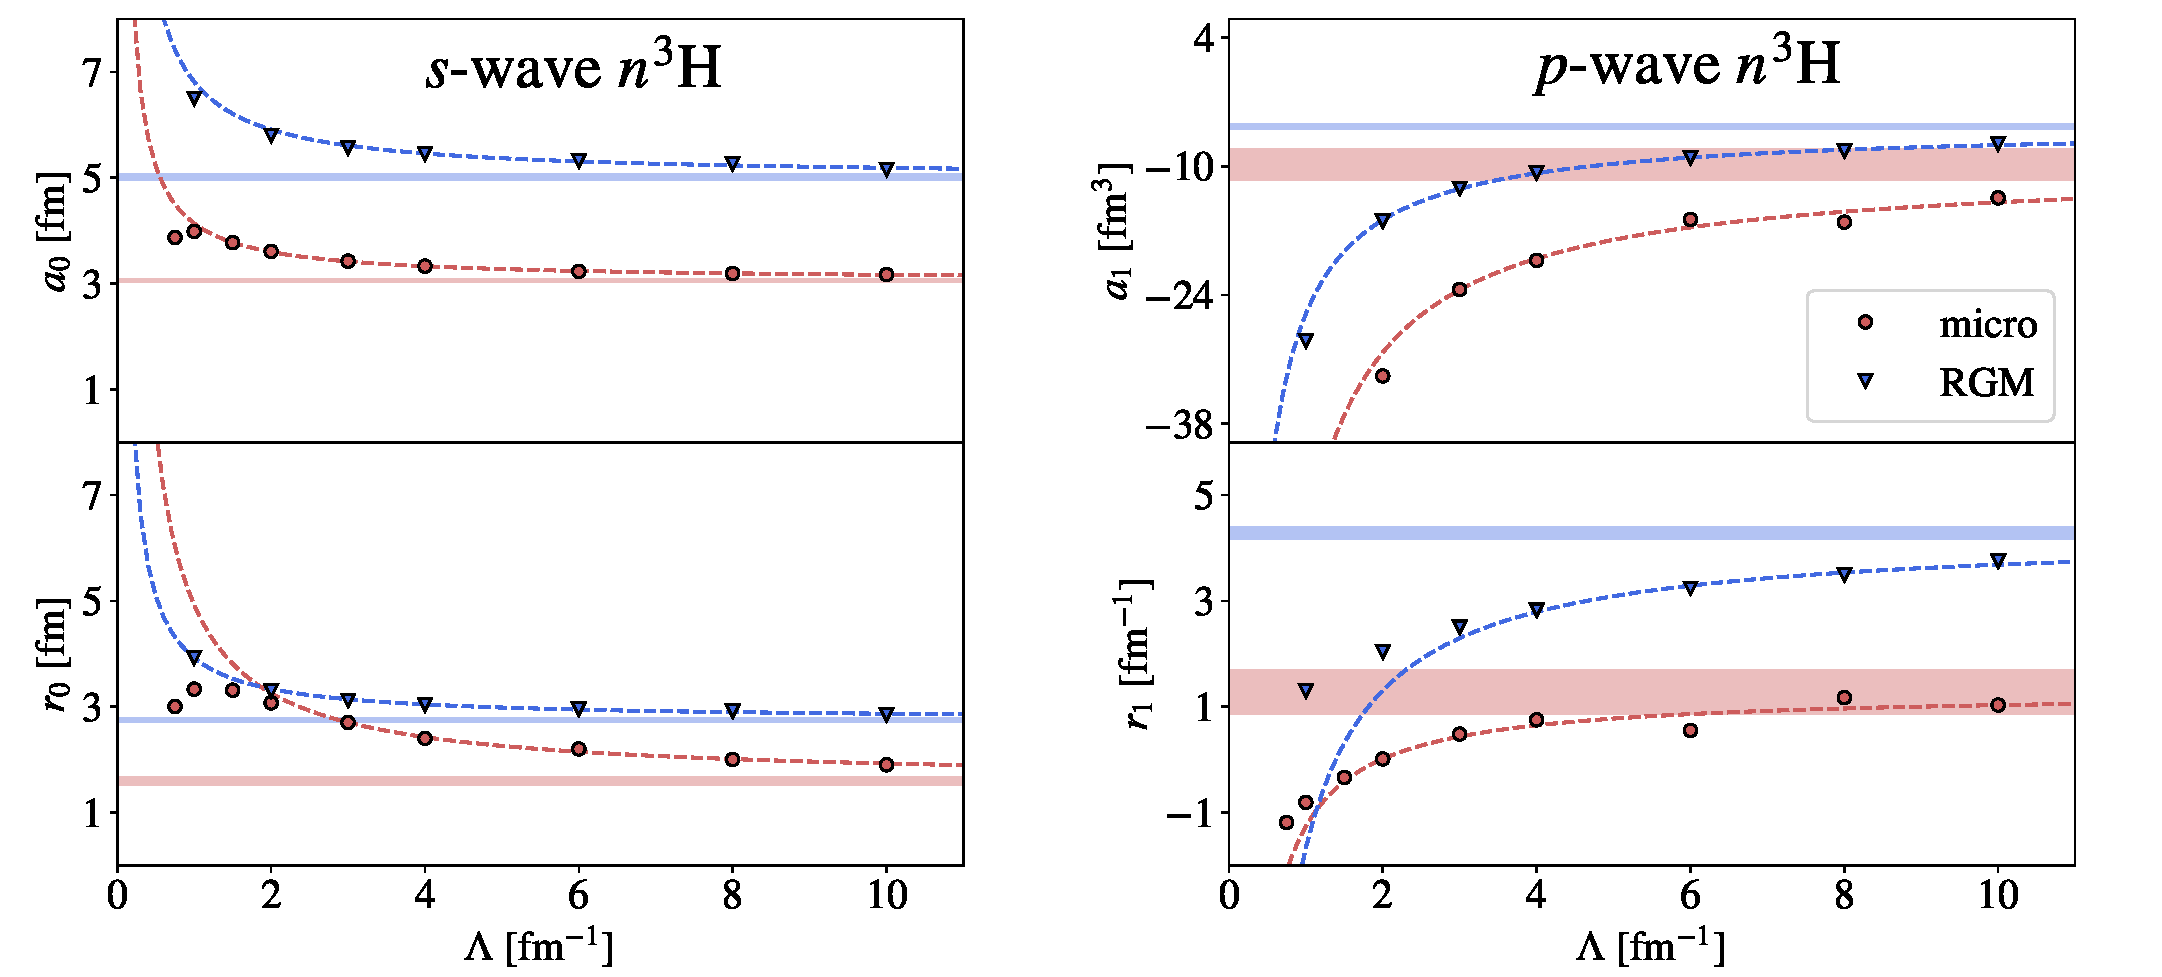
\includegraphics[width=\linewidth]{Graphs/ere.pdf}
  \caption{Left panel : $S$-wave scattering length $a_0$ and effective range $r_0$ calculated using microscopic techniques, SVM with Bush Formula and solving the Faddeev-Yakubovsky equation (red), and n$^3$H folding using RGM (blue) for the "nuclear" case. Right panel : the same as in the left panel but for $P$-wave scattering parameters - scattering volume $a_1$ and $P$-wave effective range $r_1$. For each scattering parameter the corresponding dashed line represents an extrapolation to the contact limit ($\Lambda \rightarrow \infty$) using the function in eq.~\ref{extrapolation}. The extrapolated values together with extrapolation uncertainties are shown by the shaded bands.}
  \label{fig:ERE_Parameters}
\end{figure*}


We examine the scattering parameters of the n$^3$H system calculated with the microscopic methods (SVM with Bush Formula and solving the Faddeev-Yakubovsky equation). 
For scattering lengths $a_0$ and volumes $a_1$ we find relative agreement between two microscopic methods of order $\simeq 0.1-1 \%$ for $a_0$ and $\simeq 1-10\%$ for $a_1$ between the results. 
The effective ranges in $S$-wave ($r_0$) and $P$-wave ($r_1$) were extracted only via Bush formula and their numerical errors are not larger than $0.1$~fm and $0.1$~fm$^{-1}$, respectively.

The calculated $a_0,~r_0,~a_1$,~and~$r_1$ values using ab initio methods are shown as a function of increasing momentum cut-off $\Lambda$ in fig.~\ref{fig:ERE_Parameters}. 
As expected for \eftnopi LO observables, all scattering parameters converge as $1/\Lambda$. For $\Lambda \geq 4~{\rm fm^{-1}}$ we fit corresponding values using the function
\begin{equation}
    O(\Lambda) = O(\infty) +\frac{a}{\Lambda}
    \label{extrapolation}
\end{equation}
thus extrapolating calculated scattering parameters to the contact limit ($\Lambda \rightarrow \infty$). 
The resulting values extracted within \eftnopi at LO using the ``nuclear'' parametrization are: $a_0(\infty) = 3.06(1)$~fm, $r_0(\infty) = 1.59(7)$~fm for $S$-wave and $a_1(\infty) = -9.8(1.6)$~fm$^3$, $r_1(\infty) = 1.3(4)$~fm$^{-1}$ for $P$-wave, with extrapolation errors given in parentheses.
For the ``unitary'' $NN$ case we obtain $a_0(\infty) = 2.27(1)$~fm, $r_0(\infty) = 0.47(3)$~fm for $S$-wave n$^3$H scattering and $a_1(\infty) = -5.1(1)$~fm$^3$, $r_1(\infty) = 1.8(1)$~fm$^{-1}$ for $P$-wave n$^3$H scattering. 
%
In line with the sign convention adopted in eq. \ref{eq.app.ere}, the positive $a_0$ values suggest repulsive $S$-wave interaction, indicating dominance of Pauli principle between neutrons. 
This is in agreement with the lacking of bound state solutions in the $L=0^+$ n$^3$H channel for any $\Lambda$ considered. On the other hand, negative $a_1$s for all $\Lambda$ reveal attraction in $P$-wave n$^3$-H interaction. Approaching small-$\Lambda$ region, $|a_1|$ magnitude increases and the attraction becomes stronger, eventually resulting in the appearance of one $L=1^-$ bound state below $\Lambda\simeq$0.75 fm$^{-1}$. 
It is interesting to point out that, despite $S$-wave contact nature of the LO \eftnopi theory, the n$^3$H scattering has non-zero scattering volume and range components even in the $\Lambda \rightarrow \infty$ limit.
%
Comparing the ``unitary'' with the "nuclear" cases, both repulsion in $S$-wave and attraction in $P$-wave are preserved, however, for the former, the $a_0$ and $a_1$ are smaller in magnitude, which suggests in general weaker n$ ^3$H interaction in the "unitary" case.
%
On a universal scale the scattering parameters can be expressed in
natural units of the three-body scale $R_3=1/\sqrt{-2mE_3/\hbar^2}\simeq 6$~fm: the only scale present in the system. 
In this case, the scattering parameters are reasonably natural and read $|a_0(\infty)|\simeq0.4\,R_3$, $|r_0(\infty)| \simeq 0.1\,R_3$, $|a_1(\infty)|^{1/3} \simeq 0.3\,R_3$, and $|r_1(\infty)|^{-1} \simeq 0.1\,R_3$. %** check the numbers, might be outdated **
%

%
A comparison with the experimental data and the other theoretical models can only be done in $S$-wave (no data are available for scattering volumes and ranges). However, the $a_0$ calculated with ab initio methods as well as the RGM result appears to be compatible in sign and magnitude with the realistic calculations and experimental results available (inside \eftnopi truncation error), for both the ``nuclear'' and ``unitary'' parametrization used. 
As reference for theory and experiment we use the average scattering parameters $a_0^c=\sqrt{0.25(3a_{(S=1)}^2+1a_{(S=0)}^2)}$:   $a_0^{theo}=3.71$ fm\cite{Lazauskas:2019hil} and $a_0^{exp}=2.9\,-\,4.3$ fm\cite{Tilley:1992zz}, 
which are in good agreement with \eftnopi prediction considering the LO truncation uncertainty. 
%

%
Using the RGM method, the scattering parameters found are
$a_0(\infty) = 5.71$~fm, $r_0(\infty) \simeq 0.$~fm, $a_1(\infty) = -10.49$~fm$^3$, and $r_1(\infty) = 4.33$~fm$^{-1}$ for the ``nuclear'' parametrization; and
$a_0(\infty) = 3.3$~fm, $r_0(\infty) \simeq 1.8$~fm, $a_1(\infty) = -2.5$~fm$^3$, and $r_1(\infty) = 10.1$~fm$^{-1}$ fo the ``unitary'' case. 
These results are relatively distant from the ab initio calculation, however, it is hard to estimate the error introduced by the approximations done in the method and how they correlate with the expansion parameter of the theory.
Moreover, the RGM results appear to be highly sensitive to the $^3$H wave function used in the calculation, introducing a further dependence of the results from the input choice.
The result of RGM appear also to be natural and convergent (see Fig. \ref{fig:ERE_Parameters}) in the large cut-off limit.
%maybe we can add few more comments on this, but nothing comes in my mind.

%

%
\begin{figure*}
\centering
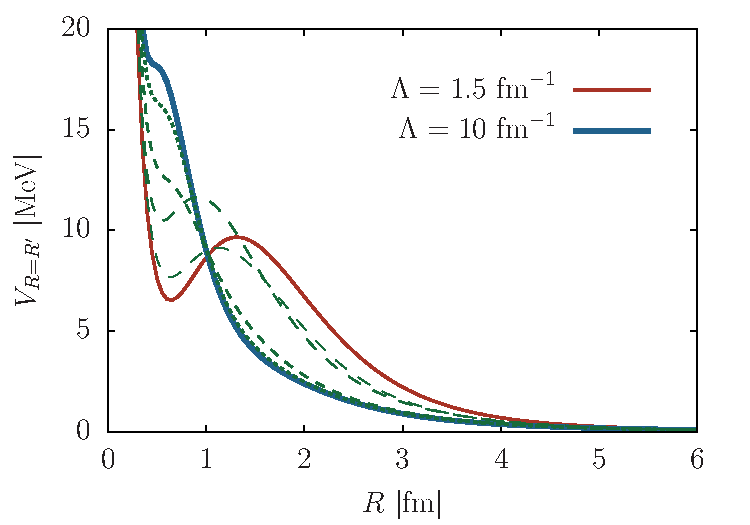
\includegraphics[width=.39\textwidth]{./Graphs/rgm_potential_unit}
\hfill
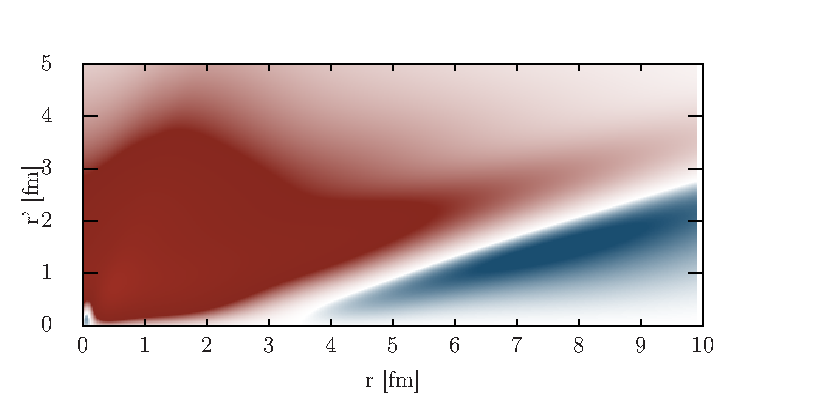
\includegraphics[width=.60\textwidth]{./Graphs/NonLocPot10_nuc}
\caption{\edit{change the capital R on left pannel and make sure it is the nuclear case}Left panel: Local part of the effective $P$-wave n$^3$H interaction $V(r,r')\delta(r'-r)$ as a function of the distance between the neutron and the center of mass of the triton. The interaction is extracted using the RGM at the n$^3$H zero energy and evaluated for different cut-offs from 1.5 (red line) to 10~fm$^{-1}$ (blue line); intermediate cut-offs are shown as green dashed lines. Right panel: Same as in the left panel but full non-local $V(r,r')$ interaction calculated for cutoff $\Lambda=10$~fm$^{-1}$.}\label{Fig:Potential}
\end{figure*}


%

%
\vspace{2mm}
%
Although the effective n$^3$H interaction is not observable, we use the RGM to extract its $P$-wave
component to acquire a deeper insight into interplay between repulsive and attractive parts and their evolution with $\Lambda$. In fig.~\ref{Fig:Potential}, we visualise such interaction for the "nuclear" case and zero-energy scattering. On the left panel, the local part of the coordinate space interaction ($r=r'$) is shown as a function of the distance between the neutron and the center of mass of the triton. 
A positive energy pocket at distance $r\simeq0.5$~fm can be noticed for small cut-offs, however, it vanishes approaching the contact limit ($\Lambda\to\infty$). On the right panel, the full coordinate interaction $V_{n-t}(r,r')$ is plotted for $\Lambda=10$~fm$^{-1}$ and zero energy. 
The non-symmetry of the interaction is a consequence of the folding technique. 
Here, the repulsive part of the interaction (red) clearly dominates and it can be traced as a combination between the repulsion induced by three-body forces, two-body exchange interaction, and centrifugal barrier. 
One can notice a weak attraction pocket ($min(V_{n-t})\approx$-0.35 MeV; blue) present far from the diagonal. 
The minimum of this pocket is too small to support a bound state, but it might be the reason for the appearance of a broad resonance state. This pocket is retained even for larger cut-offs. 

\begin{figure*}
\centering
  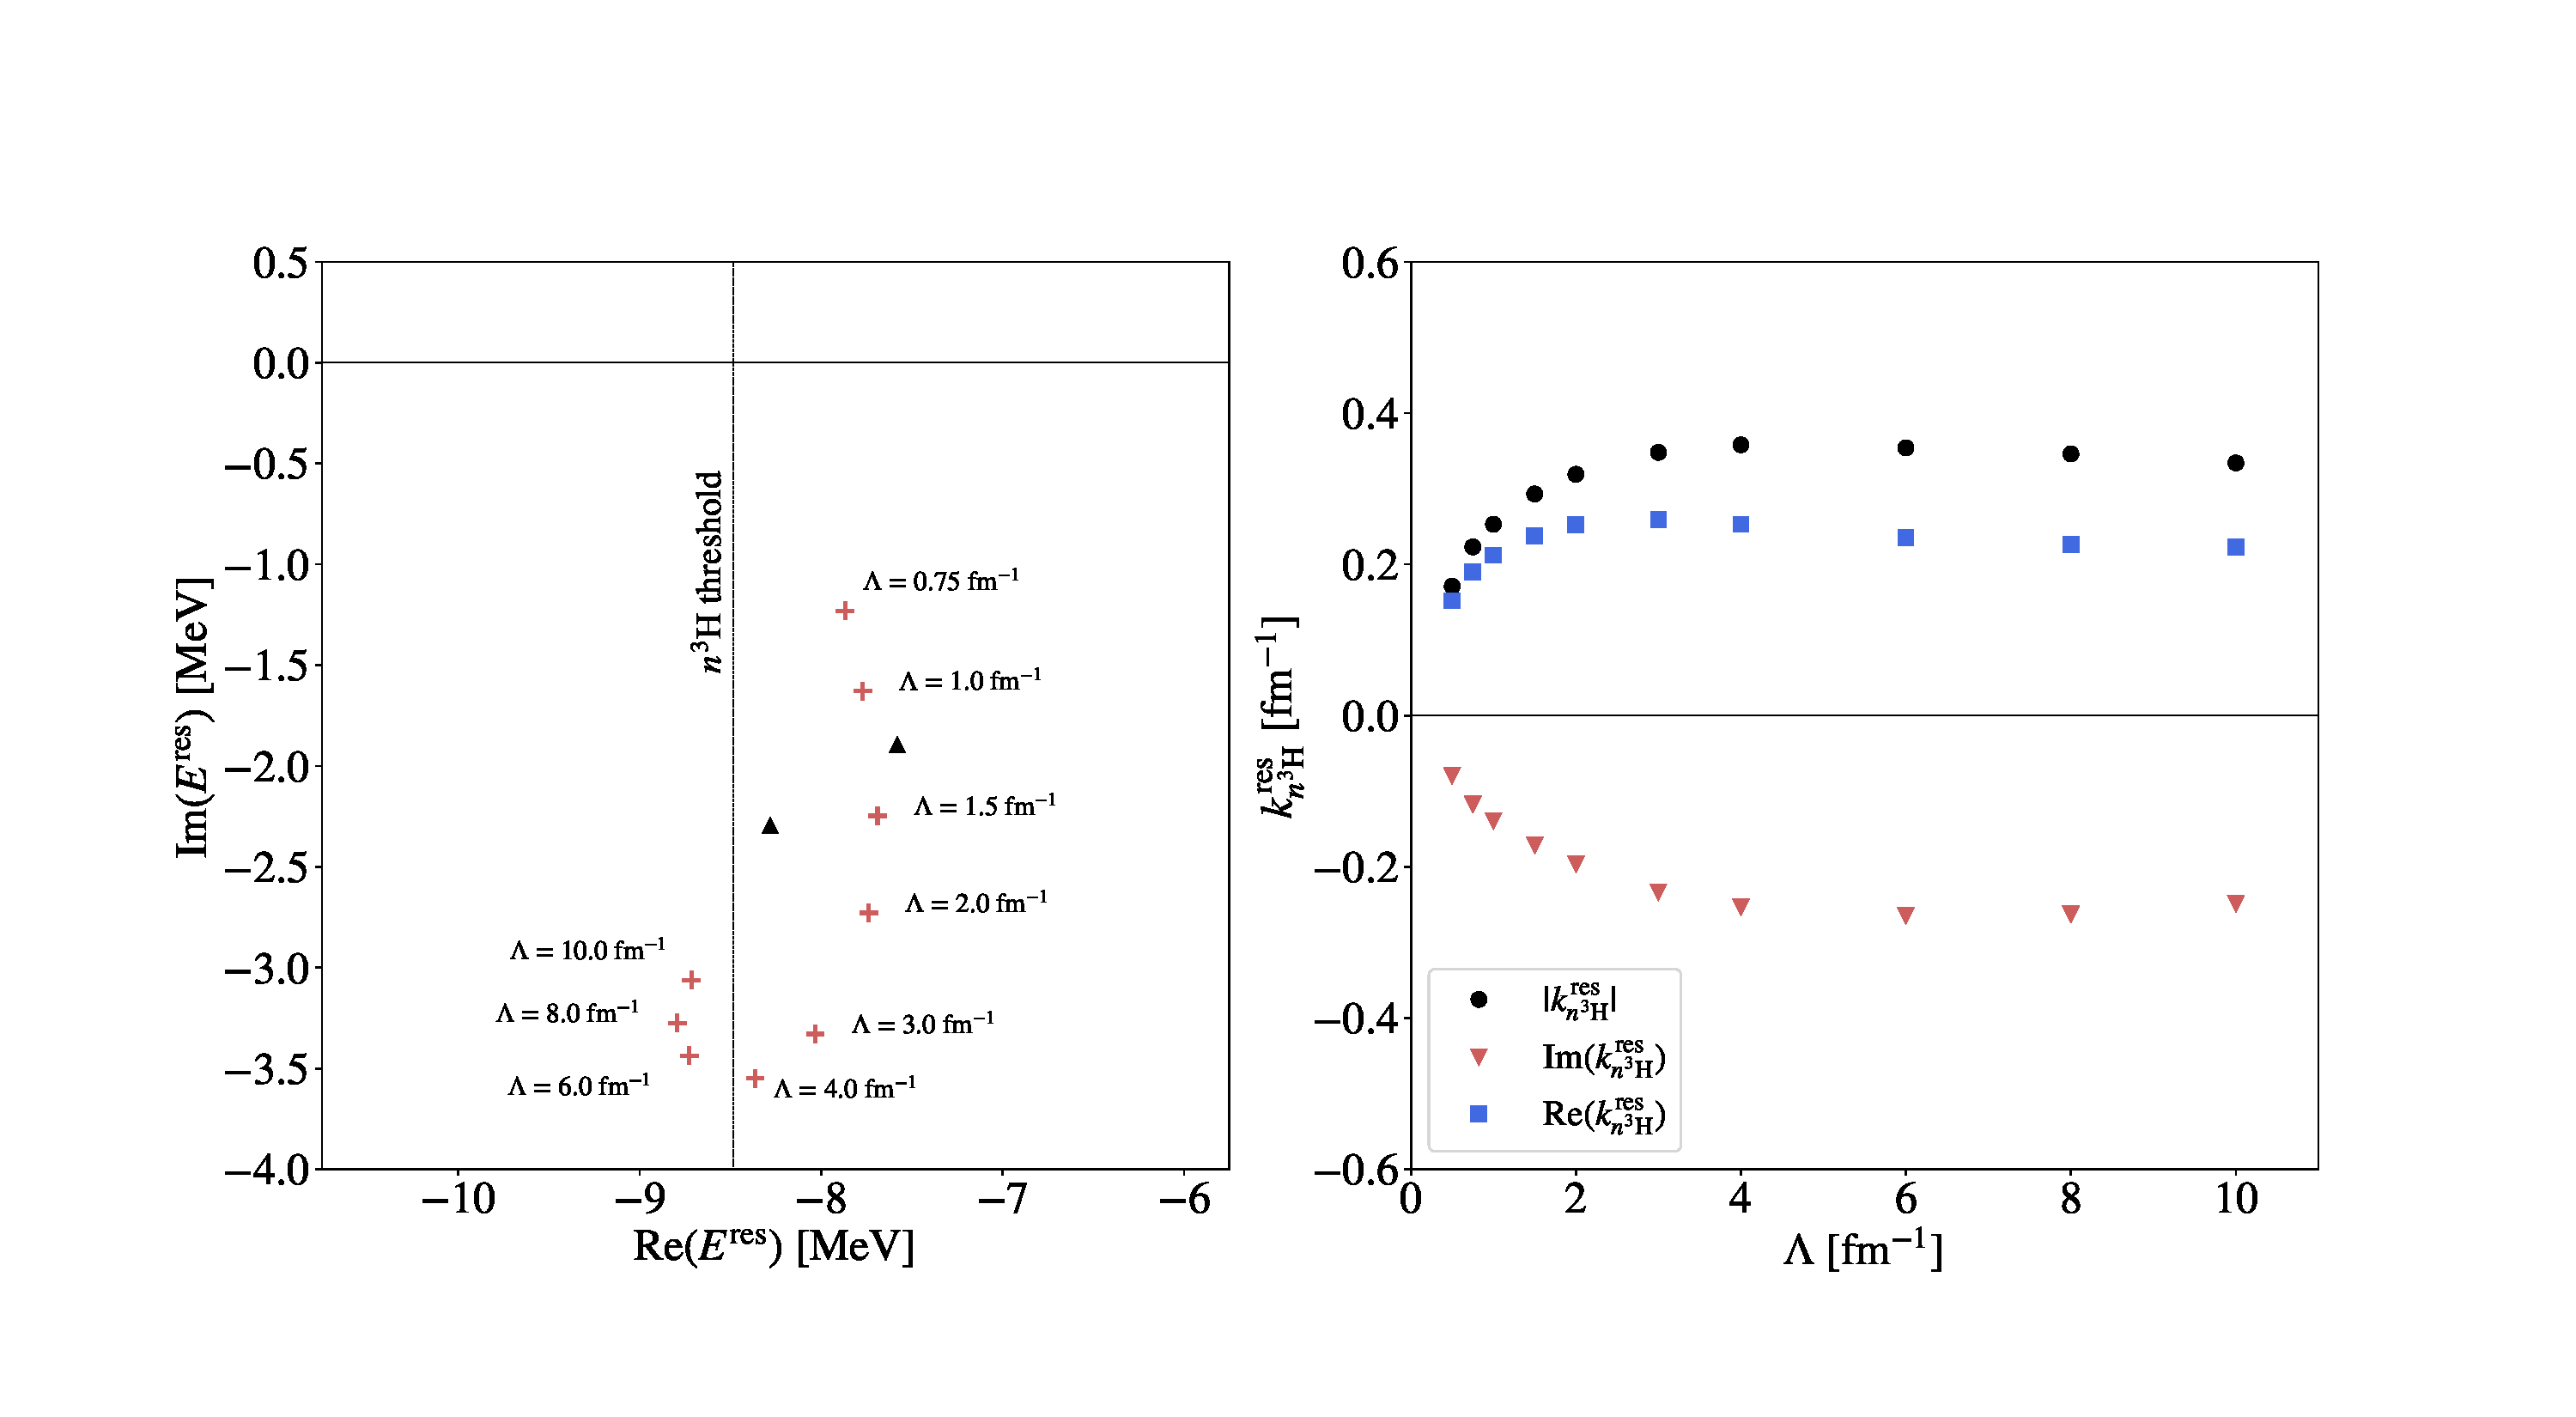
\includegraphics[width=.98\linewidth]{Graphs/resonance.pdf}
  \caption{ Left panel : Complex energy plane with calculated $^4$H $1^-$ resonance positions (red crosses) for multiple momentum cutoff $\Lambda$. 
  The black triangles represent the position of the $1^-$ resonance extracted in Ref~\cite{Lazauskas:2019cxj}
  Right panel: The absolute value, real, and imaginary part of the complex resonance momentum $k^{res}_{n ^3{\rm H}}$ as a function of increasing $\Lambda$. The momentum is related to resonance energies via eqs.~\ref{mmnt}~and~\ref{kreim}. The resonance pole was extracted directly solving the four-nucleon problem trough the Faddeev-Yakubovsky equations.}
  \label{fig:Pole_PositionN}
\end{figure*}

%
So far our calculations revealed non-vanishing $P$-wave attraction in n$^3$H scattering in the contact limit, suggested by the negative $a_1(\infty)$, and the existence of attractive pocket in the effective n$^3$H $P$-wave RGM potential which persists even at highest considered cut-off $\Lambda=10$~fm$^{-1}$. Both of these results lead us, yet still not quite firmly, to an existence of a broad $^4$H resonance stabilizing with increasing momentum cut-off. Consequently, the final step in our calculation is to search directly for a position of the $J^\pi=1^-$ nuclear resonance looking for a pole of a 4-body $S$-matrix. This has been done by solving the Faddeev-Yakubovsky equations by imposing divergent boundary conditions provided by outgoing n$^3$H wave behavior.

In the left panel of fig.~\ref{fig:Pole_PositionN}, the evolution of such pole using the ``nuclear'' interaction is shown in the complex energy plane. It can be followed to pass the n$^3$H threshold energy $B_{t}=8.484$~MeV (denoted by dashed vertical line) finally stabilizing around $E^{res}=-8.7-i\,3.1$ for cutoffs greater than $6$~fm$^{-1}$. The passage of the resonance position from the fourth quadrant (${\rm Re}(E)>0$; ${\rm Im}(E)<0$) into the subthreshold third quadrant (${\rm Re}(E)<0$; ${\rm Im}(E)<0$) makes difficult to clearly visualise the convergence of the the resonance position with increasing $\Lambda$. 
Therefore, we transform calculated resonance energies into n-$^3$H complex momenta $k^{res}_{n ^3{\rm H}}$  
\begin{equation}
    k^{res}_{n ^3{\rm H}} = \sqrt{2 \mu E^{res}_{n ^3{\rm H}}},~~~~E^{res}_{n ^3{\rm H}}= E^{res} + B_{t},
    \label{mmnt}
\end{equation}
where $\mu \approx 3/4 m$ is the reduce mass of the two-body n-$^3$H system. The real and imaginary part of the complex momentum then can be evaluated as  
\begin{equation}
    \begin{split}
        {\rm Re}(k^{res}_{n ^3{\rm H}}) &= \sqrt{\frac{2\mu \left(|E^{res}_{n ^3{\rm H}}|+{\rm Re}(E^{res}_{n ^3{\rm H}})\right)}{2}},\\
        {\rm Im}(k^{res}_{n ^3{\rm H}}) &=  {\rm sgn}\left({\rm Im}(E^{res}_{n ^3{\rm H}})\right)\sqrt{\frac{2\mu \left(|E^{res}_{n ^3{\rm H}}|-{\rm Re}(E^{res}_{n ^3{\rm H}})\right)}{2}}.\\
    \end{split}
    \label{kreim}
\end{equation}

The ${\rm Re}(k^{res}_{n ^3{\rm H}})$, ${\rm Im}(k^{res}_{n ^3{\rm H}})$, and $|k^{res}_{n ^3{\rm H}}|$ momenta are plotted as a function of $\Lambda$ in the right panel of fig.~\ref{fig:Pole_PositionN}.  
For cut-off values larger than the breakup scale of the theory $m_\pi$ the resonance momentum starts to stabilize and its absolute value $|k^{res}_{n ^3{\rm H}}|$ does not exceed $0.35~{\rm fm}^{-1}\simeq 0.5 m_\pi$, remaining well inside the convergence radius of the theory (I.e., we do not expect subleading contributions to be able to remove this state from the theory).
%

%
We notice that the resonance position can also be found as pole of the n-$^3$H T-matrix in eq. \ref{eq:Tmatrix} parametrized by the scattering parameters calculated using \eftnopi. 
Truncating the ERE at the scattering volume we expect a deviation from the \eftnopi resonant momentum of $\Gamma_{halo}$: the expansion parameter of the n-$^3$H halo EFT at the resonant energy.
Doing this exercise we find a resonant momentum of $k^{res}_{halo})\simeq80+46\,i$ MeV, which is compatible, in the truncation error of the halo EFT, with the momentum of the \eftnopi pole ($k^{res}_{n ^3{\rm H}}\simeq46+49\,i$MeV).
Confirming that the pole is also inside the convergence value and can be treated in halo EFT.  
%

%
Comparing our $^4$H resonance result with experimental data and previous calculations, the major difference is that our pole goes to the subthreshold region in the $\Lambda\rightarrow\infty$ limit, namely, the resonance energy is lower than the n$^3{\rm H}$ threshold energy (notice that this kind of states are different than boundstates and remain non normalizable).
Theoretically, this is not an issue since the pole existence in subthreshold region does not break causality and it can be moved in the standard resonant region by a continuous transformation of the interaction (e.g. reversing the renormalization group transformation) and by the inclusion of \eftnopi subleading orders. 
% I dont like this statement bc the LO is compatible with a normal resonance and we expect this pole to go in the correct physical position at a certain point in the pionless expansion
%However, such a subthreshold resonance has only small impact on the physical observables and thus its signature would be almost impossible to be detected in an experiment.
%

%
Due to the difficulty of comparing different experimental set-up and theoretical calculations, it is hard to state to which extent our $^4$H resonance calculation is in agreement with the others in quantitative terms. 
%
To stress this point, one can notice that the $S$-matrix pole energy is, in general, lower than the one extracted with $R$-matrix analysis.
An illustrative example is provided by the  transfer reactions $^2$H(t,p)$^4$H and $^3$H(t,d)$^4$H \cite{Sidorchuk:2004ntw}. 
The $R$-matrix analysis of the results obtains for the lowest $^4$H state $E_R$=3.05$\pm$0.19 MeV and $\Gamma$=4.18$\pm$1.02 MeV while the corresponding $S$-matrix pole, extracted by the same authors, led to $E_R$ =1.99$\pm$0.37 MeV and $\Gamma_R$=2.85$\pm$0.3 MeV. 
Therefore, a fair comparison can only be done with other $S$-matrix pole predicted with realistic interactions. 
%
The study done in refs~\cite{Lazauskas:2019hil,Arai:2003ek, deDiego:2007rd} found a pole corresponding to ${\rm Re}(E_r)=(0.9\,-\,1.23)$~MeV and $\Gamma=(3.5\,-\,5.8)$~MeV.
\eftnopi at LO predicts a slightly less energetic but much narrower resonance ($E_r=-0.22$~MeV and $\Gamma=1.6$~MeV). 
The maximum relative distance between the poles momentum is $\sim 80\%$ of the total energy, although a large difference, it is in line with the expected uncertainty of the powercounting truncation.
%

%
The same calculations have been repeated using the ``unitary'' $NN$ interaction. In this case, Faddeev-Yakubovsky calculations find a wider resonance than in the nuclear case at energy $E_r=-8.156$~MeV and $\Gamma=2.4$~MeV (equivalent to absolute momentum $k_{n-t}=0.58\,m_\pi$). 
Despite this pole being relatively close to the one previously calculated (40\% of relative error: in line with the SU(4) assumption expected uncertainty), it is extremely hard to be tracked and has been studied only for cut-offs compatible with $m_\pi$: $\Lambda=0.75$ and $2$ fm$^{-1}$, and was not possible to check its value in the contact limit.


%================================================
\section{Conclusions}
%================================================
%
In this work, we observe the appearance of a stable $J^{\pi}=1^-$resonance in $^4$H using the pionless effective field theory (\eftnopi) truncated at leading order. The calculation is done using microscopic ab initio techniques as well as employing a folded interaction using the resonating group method (RGM).
%
Although other works have already established the possibility of creating shallow resonances using \eftnopi in $S$-wave two-nucleons and hypernuclear systems, this is the first time a stable $P$-wave
resonance has been found within this framework. 
%The scattering observables we calculate appear to be natural when compared with the fixed three body scale.
%
To supplement our ab initio calculation, we repeated it using the RGM, fixing as calculation input the $^3$H wavefunction using the density calculated with ab initio method.
The result found for the scattering parameter are qualitatively similar, but deviate from the results calculated using ab initio methods.
However, the uncertainty of the method is hard to be estimated a priori, both for the assumption of having a frozen core $^3$H and for the sensibility to the input wave function.
Nonetheless, the RGM results appear to be cut-off convergent and natural in the contact limit.
%

%
The values of the resonance energy and of the scattering parameters extracted from $S$-matrix formalism and from experiment can be hardly compared because of the very different way of extracting them, the different interpretation of the resonant state, and the difference among the experimental setups and protocol. 
However one can compare the $S$-matrix resonant poles among different theoretical calculations. \eftnopi find a resonance that is sharper than other calculations performed with realistic interactions. However, the calculations are still in agreement considering the \eftnopi LO truncation uncertainty. Comparing the result of different parametrizations of the EFT LO, namely starting from a two-body interaction that reproduces the deuterium binding energy or from a unitary interaction, we find a difference that is again in agreement with the expected uncertainty given by assuming a spin-independent interaction.
%
On the qualitative point of view, the major difference between \eftnopi and the resonances found in literature is the subthreshold nature (the resonance energy is lower than the threshold energy) of the former. 
However, this is not fundamentally a problem, in part because these pole can be physical\cite{formartinanyexample}, and because a non-subtreshold resonance may still be obtained introducing orders of the EFT expansion.
%

%
The possibility of creating $P$-wave many-body poles using a contact $S$-wave theory is remarkable in itself, but it also has strong implications for \eftnopi powercounting, possibly solving the issue of the absence of stable bound states states for nuclei larger than $^4$He at LO. We conjecture that an existing $P$-wave resonance might be moved on the stable region by the insertion of sub-leading orders, which would be trivially impossible if no $P$-wave states are present at all.

\section*{acknowledgement}
We thank Bira van Kolck for the patience, discussions, and mentoring about \eftnopi and halo EFT. 
MS was supported by the Pazy Foundation and the Israel Science Foundation grant 1086/21.
JK acknowledges the hospitality and support of The George Washington University and the helpful
conversations with H.~W.~Grie\ss hammer and N.~Walet.
LC an JC supported in part by the National Science Foundation under Grant No. NSF PHY-1748958.



\bibliographystyle{ieeetr}

%elsarticle-harv}
\bibliography{bibi.bib}

\end{document}